\chapter{Fundamentos de las redes neuronales} \label{Capitulo_2}


 

\section{Revisión teórica} \label{Subsec: 3_1}
Puedo introducir los tipos de funciones de activavion. Esta bien explicado en el TFG wuolah o en el articulo de KDD cup 199 de DNN network intrusion.
Puedo añadir overfitting y underfitting.
lo que es aprendizaje supervisado y no supervisao
Partes de una neurona y como trabaja(bias, pesos...)


\section{Arquitecturas relevantes} \label{Subsec: 3_2}
Mini tabla resumen en Deep Cybersecurity: A Comprehensive Overview from Neural Network and Deep Learning Perspective y miniresumen de todos los tipos en review Deep Cybersecurity: A Comprehensive Overview from Neural Networkand Deep Learning Perspective y review
\subsection{Autoencoder}

Leer y sacar la información del word autoencoders.

Los autoencoders son una clase de redes neuronales artificiales utilizadas en aprendizaje no supervisado para aprender representaciones eficientes de datos. Su objetivo principal es codificar la entrada en una representación comprimida y significativa, y luego decodificarla de manera que la reconstrucción sea lo más similar posible a la entrada original.

La arquitectura básica de un autoencoder consta de dos partes: el encoder y el decoder. El encoder mapea los datos de entrada a una representación oculta de menor dimensión utilizando funciones principalmente no lineales, mientras que el decoder reconstruye los datos de entrada a partir de esta representación oculta. Durante el entrenamiento, los parámetros del autoencoder se optimizan para minimizar la diferencia entre la entrada y la salida reconstruida, utilizando una función de pérdida que mide esta discrepancia.

Los autoencoders se han utilizado en una amplia variedad de aplicaciones, incluida la reducción de dimensionalidad, la extracción de características, la eliminación de ruido en los datos de entrada y la detección de anomalías. Su versatilidad y capacidad para aprender representaciones útiles de los datos los hacen herramientas poderosas en el campo del aprendizaje automático y la inteligencia artificial.



\subsection{Deep Belief Networks}
\subsubsection{Red Neuronal Profunda}
\subsection{Red Neuronal Convolucional}
\subsection{Red Neuronal Recurrente}
\subsubsection{Restricted Boltzmann Machine}


\section{Implementación en Python} \label{Subsec: 3_3}
\subsection{Frameworks}

numpy
matplotlib
sklearn

\subsubsection{Deep neural network}

\section{Principales Deep Learning Frameworks. Keras.}

\begin{wrapfigure}{r}{0.33\textwidth}
  \begin{center}
    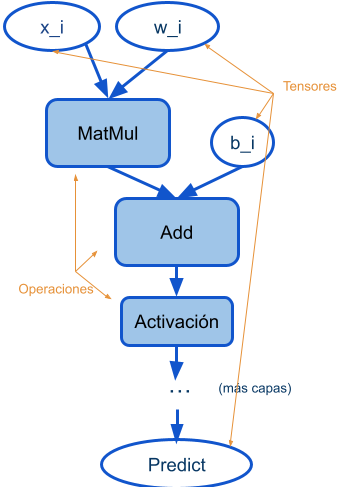
\includegraphics[width=0.33\textwidth]{img/graficoTF.png}
  \end{center}
    \caption{Gráfico de una red neuronal.}
  \label{fig:graficoTF}
\end{wrapfigure}
\vspace{-\baselineskip}

A medida que las técnicas de aprendizaje profundo han ido ganando popularidad, muchas organizaciones académicas e industriales se han centrado en desarrollar marcos de trabajo para facilitar la experimentación con redes neuronales profundas de manera sencilla para el usuario. En esta sección, ofrecemos una visión general de los bibliotecas más conocidss: TensorFlow, PyTorch y Keras.

 
\textbf{TensorFlow} \citep{tensorflow} es una biblioteca de código abierto que fue desarrollada en 2016 por el equipo de Google Brain del departamento de IA de Google. Es una plataforma que se centra principalmente en el aprendizaje automático y la computación de alto rendimiento. Su modelo de programación permite que los datos fluyan de una operación a otra de manera flexible gracias a su estructura de grafo computacional y al concepto de flujo de datos. Los gráficos son estructuras de datos que contienen un conjunto de objetos tf.Operation (nodos), que representan unidades de cálculo y objetos tf.Tensor \footnote{arreglos multidimensionales que pueden contener datos de cualquier tipo y forma}, que representan las unidades de datos que fluyen entre esas operaciones (Figura \ref{fig:graficoTF}). Esto permite una ejecución eficiente y paralela de operaciones en diferentes dispositivos de hardware, como en una CPU, GPU, dispositivos móviles y sistemas distribuidos a gran escala con cientos de nodos. Esta flexibilidad y además su capacidad de diferenciación automática lo hacen una biblioteca útil para una gran variedad de aplicaciones, desde la investigación hasta el desarrollo y la producción de modelos de aprendizaje automático.





\textbf{PyTorch} \citep{pytorch}, presentado por el equipo de investigación en IA de Facebook en 2016, es una biblioteca de aprendizaje profundo desarrollado en Python que simplifica la creación de modelos complejos a través de una interfaz de programación sencilla. A diferencia de otros marcos populares que emplean gráficos de computación estáticos, PyTorch se basa en la computación dinámica (su topología puede variar durante la ejecución del programa), lo que permite una mayor flexibilidad para diseñar arquitecturas complejas. Cambiar el comportamiento de una red neuronal típicamente implica reiniciar desde cero, pero PyTorch emplea una técnica llamada auto-diferenciación en modo inverso, que permite realizar cambios en el comportamiento de la red con poco esfuerzo. PyTorch se ha vuelto popular tanto en la comunidad científica como en la industria debido a su facilidad de uso y su capacidad para crear modelos complejos de manera eficiente. Además, ha sido adoptado por varias organizaciones importantes, incluidas Facebook, Twitter y NVIDIA, lo que garantiza su continuo desarrollo y soporte.


\textbf{Keras} \citep{keras} es un marco de redes neuronales de código abierto desarrollado por François Cholle, un miembro del equipo de IA de Google. Se considera un meta-marco de trabajo que interactúa con otros marcos. En particular puede ejecutarse en la parte superior de TensorFlow y Theano. Está implementado en Python y proporciona APIs de redes neuronales de alto nivel para desarrollar modelos de aprendizaje profundo. En lugar de manejar operaciones de bajo nivel (diferenciación y manipulación de tensores), Keras depende de una biblioteca especializada que sirve como su motor de backend. Keras minimiza el número de acciones requeridas por un usuario para una acción específica. Una característica importante de Keras es su facilidad de uso sin sacrificar la flexibilidad. Keras permite a los usuarios implementar sus modelos como si estuvieran implementados en los marcos base (como TensorFlow o Theano\footnote{Librería de Python para aprendizaje automático.}). Proporciona un rendimiento y escalabilidad de nivel industrial, siendo utilizado por organizaciones de renombre como NASA, YouTube y Waymo para una amplia gama de aplicaciones en inteligencia artificial y aprendizaje automático.


Analizando los resultados de \citep{mahmoud2019dlbench}, podemos observar que usando la CPU, Keras destaca por encima de las demás. No solo logra el mejor accuracy en los tres datasets (MNIST, CIFAR-10, CIFAR-100), sino que además también tiene los tiempos de ejecución más bajos y una de las mejores tasas de convergencia. Estos datos sobresalientes además de su facilidad de uso, accesibilidad y documentación bien estructurada han sido determinantes para acabar por decantarme por Keras. Según Aakash Nain \citep{keraswebsite2} \begin{quote} Keras is that sweet spot where you get flexibility for research and consistency for deployment. Keras is to Deep Learning what Ubuntu is to Operating Systems. \end{quote}

y según Matthew Carrigan \citep{keraswebsite} \begin{quote}The best thing you can say about any software library is that the abstractions it chooses feel completely natural, such that there is zero friction between thinking about what you want to do and thinking about how you want to code it. That's exactly what you get with Keras.\end{quote}

\begin{comment}

\textbf{MXNet} \citep{mxnet} es un marco de trabajo de aprendizaje profundo de código abierto fundado como una colaboración entre la Universidad Carnegie Mellon, la Universidad de Washington y Microsoft. Es una librería escalable que permite el entrenamiento de redes neuronales profundas utilizando diferentes lenguajes de programación, incluyendo C++, Python, MATLAB, JavaScript, R, Julia y Scala. MXNet incluye la interfaz de Gluon que permite a los desarrolladores con cualquier nivel de experiencia comenzar a usar el aprendizaje profundo en la nube, en dispositivos de borde \footnote{dispositivos más cercanos al usuario, como teléfonos móviles, sistemas ciberfísicos (CPS), dispositivos portátiles, IoT, \ldots.} y en aplicaciones para dispositivos móviles. MXNet admite además el paralelismo de datos en múltiples CPUs o GPUs, así como el paralelismo de modelos. Ofrece dos modos de entrenamiento diferentes: síncrono y asíncrono \footnote{síncrono: interactúan en el mismo momento en el que tiene lugar la comunicación; asíncrono: la interacción no es inmediata y puede tener lugar en momentos diferentes} y además proporciona operaciones primitivas de tolerancia a fallas a través de guardar y cargar: guardar almacena los parámetros del modelo en un archivo de punto de control y cargar restaura los parámetros del modelo desde un archivo de punto de control. MXNet admite tanto la programación declarativa como la programación imperativa.
\textbf{Theano} \citep{theano} es una biblioteca de Python de código abierto para cálculos a gran escala que ha sido desarrollado por investigadores y desarrolladores de la Universidad de Montreal. Es una biblioteca que facilita la construcción de modelos de aprendizaje profundo y se puede ejecutar en diferentes plataformas informáticas, incluyendo CPU y GPU. Los cálculos se expresan utilizando una sintaxis similar a la de Numpy y funciona creando una representación simbólica de las operaciones que se traducen a C++ y luego se compilan en moléculas Python. Theano admite tanto el paralelismo de datos como el paralelismo de modelos.
\textbf{Chainer} \citep{chainer} es un marco de aprendizaje profundo de código abierto implementado en Python. El desarrollo de Chainer está liderado por investigadores y desarrolladores de la Universidad de Tokio. Chainer proporciona APIs de diferenciación automática para construir y entrenar redes neuronales, con un enfoque de ``definir por ejecutar'', lo que permite construir el grafo computacional durante el entrenamiento y permite al usuario cambiarlo en cada iteración. Chainer es un marco flexible ya que proporciona una API imperativa en Python y NumPy. Se admiten tanto cálculos en CPU como en GPU.
\end{comment}









